\section*{Lecture 17}

\subsection*{1.} Consider the ODE
\[ 
y''(t) + 3y'(t) + y(t) = y'(t)^2
.\]

\paragraph{(a)} Rewrite the ODE as a system of first order ODEs.
\bigbreak
We start by defining:
\begin{align*}
  y_1(t) &= y(t) \\
  y_2(t) &= y'(t) \\
.\end{align*}
And now we get the system of nonlinear ODEs:
\begin{align*}
  y_1'(t) &= y_2(t) = f_1(y_1(t), y_2(t))\\
  y_2'(t) &= - y_1(t) - 3y_2(t) y_2(t)^2 = f_2 \left( y_1(t), y_2(t) \right)
.\end{align*}



\paragraph{(b)} Find the location of all critical points.
\bigbreak
We can find the location of the critical points as:
\[ 
\frac{\mathrm{d}y_2}{\mathrm{d}y_1} = \frac{y_2'(t) \, \mathrm{d}t}{y_1'(t) \, \mathrm{d}t } = \frac{y_2'(t)}{y_1'(t)} = \frac{f_2(y_1(t), y_2(t))}{f_1(y_1(t), y_2(t))} = \frac{0}{0} \implies y_1 = y_2 = 0
.\]
This means we have a single critical point at $(0,0)$.

\paragraph{(c)} Linearise the system of ODEs in (a) around the critical points and determine the type/stability properties of the critical points of the linearised system.
\bigbreak
We start by calculating the Jacobian (linearization matrix) at the critical point:
\begin{align*}
  \frac{\partial f_1}{\partial y_1} &= 0 \\
  \frac{\partial f_1}{\partial y_2} &= 1 \\
  \frac{\partial f_2}{\partial y_1} &= -1 \\
  \frac{\partial f_2}{\partial y_2} &= 2y_2 - 3, \left( y_1, y_2 \right) = \left( 0,0 \right) \implies 2y_2 - 3 = -3
.\end{align*}
Therefore the Jacobian is:
\[ 
A = \begin{pmatrix}
0 & 1\\
-1 & -3\\
\end{pmatrix}
.\]
We must now find the eigenvalues of this Jacobian $A$ as:
\[ 
\mathrm{det}(A - \lambda I) = \left| \begin{array}{cc}
-\lambda & 1\\
-1 & -3 - \lambda\\
\end{array} \right| = \left( -\lambda \right) \left( -3 -\lambda \right) - 1 = 0 \implies \lambda_1 = \frac{-3+\sqrt{5}}{2}, \lambda_2 = \frac{-3-\sqrt{5}}{2}
.\]
We can now define:
\begin{align*}
  p &= \lambda_1 + \lambda_2 = -3 \\
  q &= \lambda_1 \lambda_2 = 1\\
  \Delta &= \left( \lambda_1 - \lambda_2 \right)^2 = 5
.\end{align*}
Therefore we have a stable and attractive node at the critical point.




\subsection*{2.} Consider the ODE
\[ 
y''(t) - y(t) = y(t)^2
.\]

\paragraph{(a)} Rewrite the ODE as a system of first order ODEs.
\bigbreak
We start by defining:
\begin{align*}
  y_1(t) &= y(t) \\
  y_2(t) &= y'(t)
.\end{align*}
And now we get the system of nonlinear ODEs:
\begin{align*}
  y_1'(t) &= y_2(t) = f_1 \\
  y_2'(t) &= y_1(t)^2 + y_1(t) = f_2
.\end{align*}


\paragraph{(b)} Find the location of all critical points.
\bigbreak
We can find the locations of the critical points as:
\[ 
  \frac{\mathrm{d}y_2}{\mathrm{d}y_1} = \frac{f_2}{f_1} = \frac{0}{0} \implies y_2 = 0, y_1 = \{-1,0\} 
.\]
Therefore the critical points are at $\left( 0,0 \right) $ and at $\left( -1,0 \right) $


\paragraph{(c)} Linearise the system of ODEs in (a) around the critical points and determine the type/stability properties of the critical points of the linearised system.
\bigbreak
We start by calculating the Jacobian $A$ at $(0,0)$ as:
\begin{align*}
  \frac{\partial f_1}{\partial y_1} &= 0 \\
  \frac{\partial f_1}{\partial y_2} &= 1 \\
  \frac{\partial f_2}{\partial y_1} &= 1 \\
  \frac{\partial f_2}{\partial y_2} &= 0 \\
  \implies A &= \begin{pmatrix}
  0 & 1\\
  1 & 0\\
  \end{pmatrix}
.\end{align*}
We can now find the eigenvalues of this Jacobian as:
\[ 
\mathrm{det}(A - \lambda I) = \left| \begin{array}{cc}
-\lambda & 1\\
1 & -\lambda\\
\end{array} \right| = \left( -\lambda \right)^2 - 1 = 0 \implies \lambda_1 = 1, \lambda_2 = -1
.\]
We can now define:
\begin{align*}
  p &= \lambda_1 + \lambda_2 = 0\\
  q &= \lambda_1 \lambda_2 = -1 \\
  \Delta &= \left( \lambda_1 - \lambda_2 \right)^2 = 0
.\end{align*}
Therefore we have an unstable saddle point at $(0,0)$.

For the critical point at $(-1,0)$ we change the coordinates such that the critical point is placed in $(0,0)$ in the $\tilde{y}_1\tilde{y}_2$-coordinate system. This is done as:
\begin{align*}
  \tilde{y}_1 &= y_1 + 1 \\
  \tilde{y}_2 &= y_2
.\end{align*}
The new system of first order ODEs therefore becomes:
\begin{align*}
  \tilde{f}_1 &= \tilde{y}_2 \\
  \tilde{f}_2 &= \left( \tilde{y}_1 - 1 \right)^2 + \left( \tilde{y}_1 - 1 \right)
.\end{align*}
We can now calculate a Jacobian $B$ for these at $\left( \tilde{y}_1, \tilde{y}_2 \right) = \left( 0,0 \right) $ as:
\begin{align*}
  \frac{\partial \tilde{f}_1}{\partial \tilde{y}_1} &= 0 \\
  \frac{\partial \tilde{f}_1}{\partial \tilde{y}_2} &= 1 \\
  \frac{\partial \tilde{f}_2}{\partial \tilde{y}_1} &= -1 \\
  \frac{\partial \tilde{f}_2}{\partial \tilde{y}_2} &= 0 \\
  \implies B &= \begin{pmatrix}
  0 & 1\\
  -1 & 0\\
  \end{pmatrix}
.\end{align*}
We can find the eigenvalues of this as:
\[ 
\mathrm{det}(B - \lambda I) = \left| \begin{array}{cc}
-\lambda & 1\\
-1 & -\lambda\\
\end{array} \right| = \left( -\lambda \right)^2 + 1 = 0 \implies, \lambda_1 = -i, \lambda_2 = i
.\]
We can now define:
\begin{align*}
  p &= 0 \\
  q &= 1 \\
  \Delta &= -4
.\end{align*}
Therefore we have a stable centre at $\left( \tilde{y}_1, \tilde{y}_2 \right) = (0,0) \implies \left( y_1, y_2 \right) = \left( -1, 0 \right) $

\subsection*{3.} Consider the nonlinear system of first order ODEs
\begin{align*}
  y_1'(t) &= e^{y_2(t)} -1 \\
  y_2'(t) &= 2 e^{y_1(t)} + y_2(t) - 2
.\end{align*}

\paragraph{(a)} Find the location of all critical points.
\bigbreak
We can find the locations of the critical points as:
\[ 
\frac{\mathrm{d}y_2}{\mathrm{d}y_1} = \frac{f_2}{f_1} = \frac{0}{0} \implies y_1 = y_2 = 0
.\]
Therefore there is a critical point at $\left( 0,0 \right) $.


\paragraph{(b)} Linearise the system of nonlinear ODEs around the critical points and determine the type/stability properties of the critical points of the nonlinear system.
\bigbreak
We start by calculating the Jacobian $A$ at $(0,0)$ as:
\begin{align*}
  \frac{\partial f_1}{\partial y_1} &= 0 \\
  \frac{\partial f_1}{\partial y_2} &= 1 \\
  \frac{\partial f_2}{\partial y_1} &= 2 \\
  \frac{\partial f_2}{\partial y_2} &= 1 \\
  \implies A &= \begin{pmatrix}
  0 & 1\\
  2 & 1\\
  \end{pmatrix}
.\end{align*}
Therefore we can see from Exercise 5 in Lecture 16 that we have an unstable saddle point at $(0,0)$.


\paragraph{(c)} Sketch the phase portrait of the nonlinear system close to its critical points.

\textit{Hint:} You may want to use Exercise 5, Lexture 16.
\bigbreak
In Exercise 5 from Lecture 16 this phase portrait was produced:
\begin{figure} [ht]
  \centering
  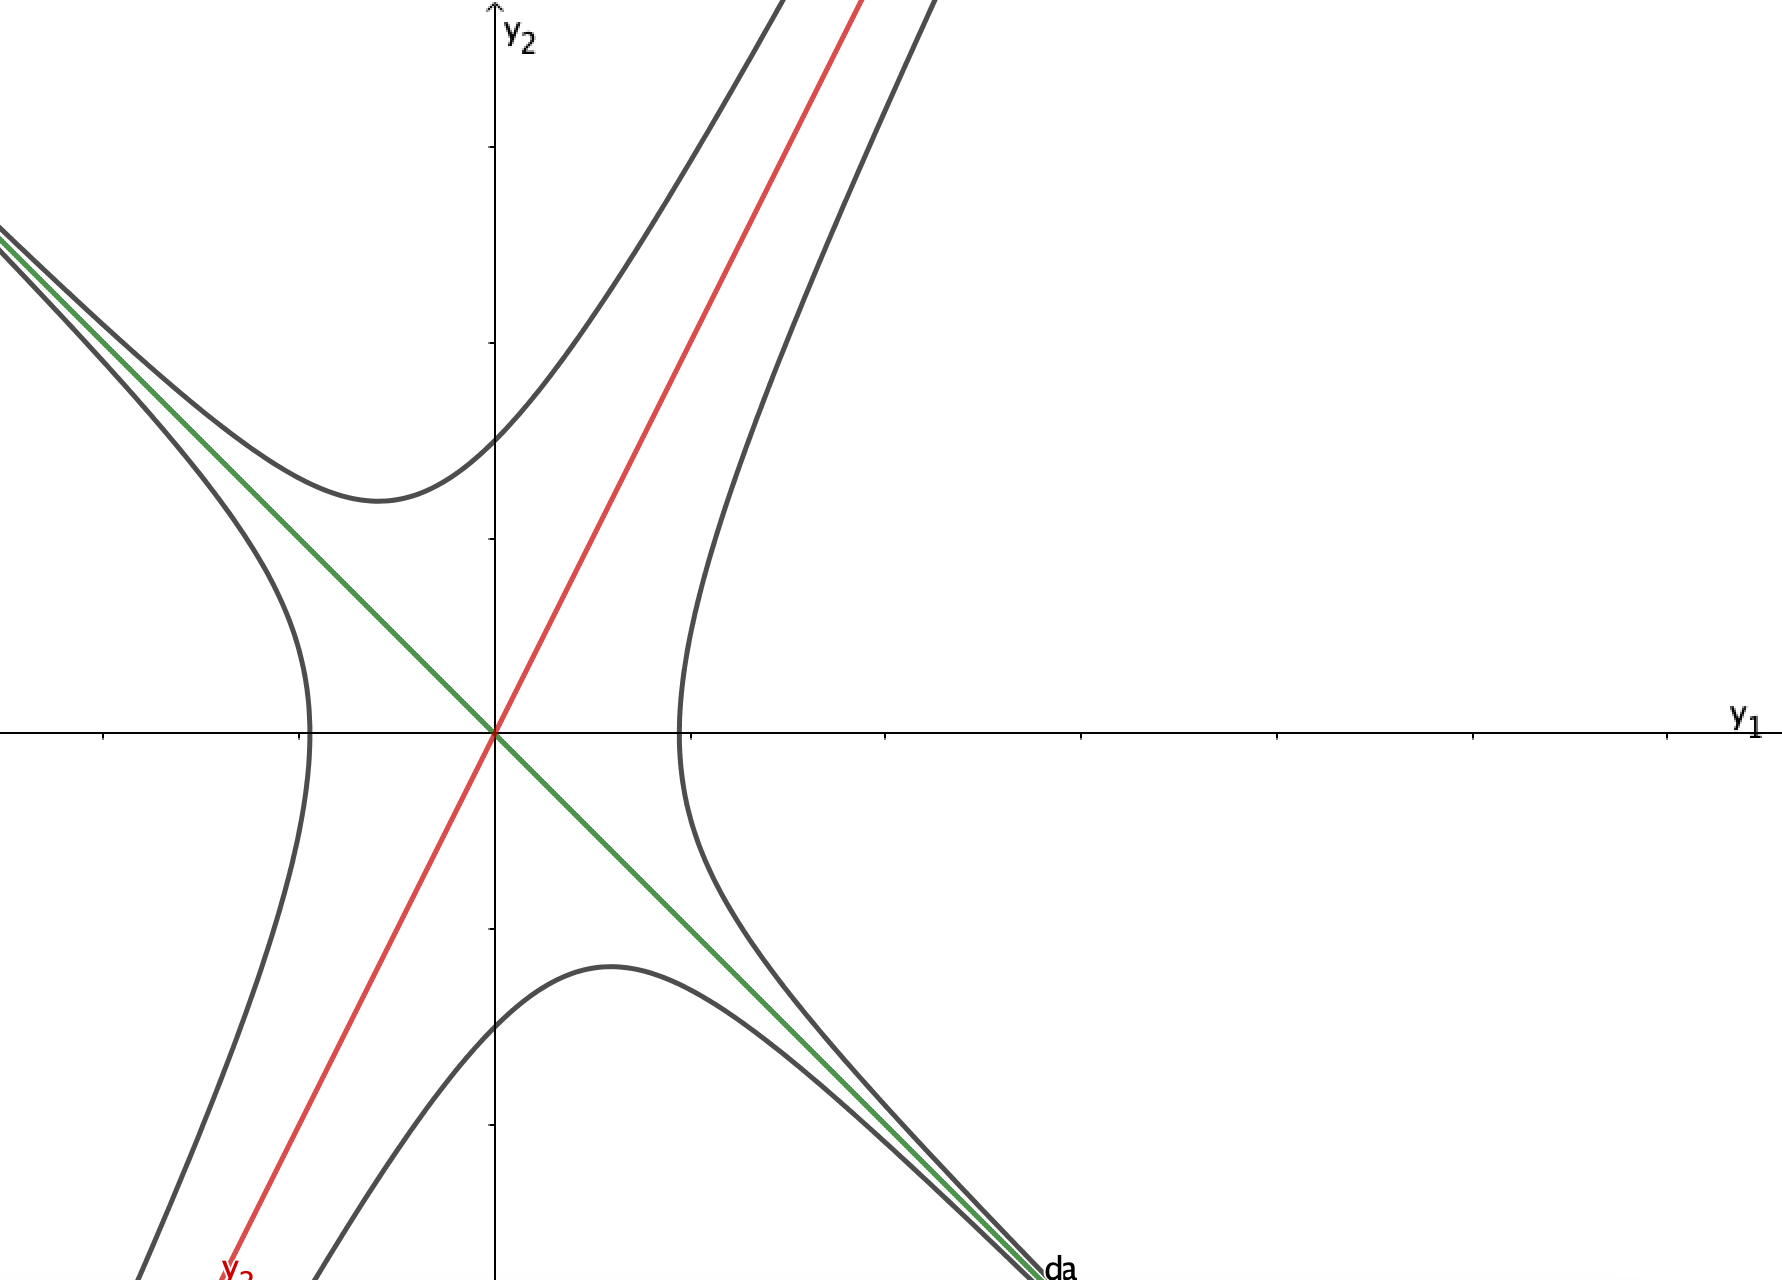
\includegraphics[width=0.5\linewidth]{./figures/e16_5.png}
  \caption{}
  \label{fig:e16_5_2}
\end{figure}
The figure on \textbf{\autoref{fig:e16_5_2}} is also the solution to this exercise.
